\documentclass[12pt,a4paper]{article}
\usepackage{hyperref}
\usepackage{graphicx}
\title{Laboratory 2: Unauthorized Access in Wireless Networks}
\author{Niclas Scheuing and Vasileios Dimitrakis}
\begin{document}
\maketitle

\section{Introduction}
	In this laboratory exercise, we learn about and experiment on the weakness in various wireless security mechanisms. More specifically, in the first chapter, we hack the MAC filtering, in the second one, we crack the WEP encryption and in the last part, we break the WPA2 Personal Passwords.

\section{Materials and Methods}
Throughout the lab exercise 2 we used different materials and methods, that are presented below:

\begin{itemize}
	\item \emph{ifconfig}: Is used to configure the network interfaces.
	\item \emph{hostapd}: Is a user space deamon for Access Point and authentication servers.
	\item \emph{iwconfig}: Is used to configure the wireless network interfaces.
	\item \emph{iwlist}: Is used to display some additional information from a wireless network interface that is not displayed by iwconfig
	\item \emph{wireshark}: Is an open source packet analyser.
	\item \emph{macchanger}: Is a Linux command that changes the MAC address of a network interface.
	\item \emph{airodump-ng}: Is used for packet capturing of raw 802.11 frames and is particularly suitable for collecting WEP IVs (Initialization Vector) for the intent of using them with aircrack-ng.
	\item \emph{aircrack-ng}: Is an 802.11 WEP and WPA-PSK keys cracking program that can recover keys once enough data packets have been captured.
	\item \emph{ping}: Is a computer network administration software utility used to test the reachability of a host on an Internet Protocol (IP) network and to measure the round-trip time for messages sent from the originating host to a destination computer and back.
	\item \emph{wpa\_supplicant}: Is a cross-platform supplicant with support for WEP, WPA and WPA2.
	\item \emph{aireplay-ng}: Inject ARP-request packets into a wireless network to generate traffic.
\end{itemize}

\section{Terminology}
The machine serving as wireless nodes is denoted by \emph{User} and the machine used to attack the communication by \emph{Attacker}.
The machine used as access point is called \emph{AP} in the following.


\section{Experiments}
  In the following we will go through the experiments one by one and introduce the corresponding theory, setup and results.
  \subsection{Hacking MAC Filtering}
	  \emph{MAC} filtering is a security technique to prevent unauthorized users from accessing a wireless network.
	  All network devices have a unique 48bit \emph{MAC} address.
	  The access-point grants or denies access to devices based on the \emph{MAC} address communicated by the device itself. This is why a device can spoof the \emph{MAC} address.
	  For filtering black-lists and white-lists are used, granting access to devices contained in the white-list and denying access to those in the black-list.
	  
  \subsubsection{Running the Experiment}
	\emph{AP} used a white-list containing the \emph{User's} \emph{MAC} address, but not the \emph{Attacker's}.
	The \emph{AP} and the \emph{User} were transmitting data.
	The \emph{Attacker} was not able to connect to the \emph{AP}, because he was not on the white-list.
	
	To find the channel and \emph{AP's} \emph{MAC}, the \emph{Attacker} used the \emph{iwlist} tool.
	The \emph{Attacker} is observing the communication running its Wifi adapter in \emph{monitor} mode and capturing the observed traffic with \emph{Wireshark}. This way he was able to extract the \emph{User's} \emph{MAC}. See \autoref{mac:wireshark}
	
	Knowing this \emph{MAC}, the \emph{Attacker} sets his own \emph{MAC} address to the \emph{User's} address using the \emph{macchanger} tool. See \autoref{mac:changer}.
	The \emph{Attacker} \emph{User} were then able to connect to the \emph{AP}.
		
	\begin{figure}
		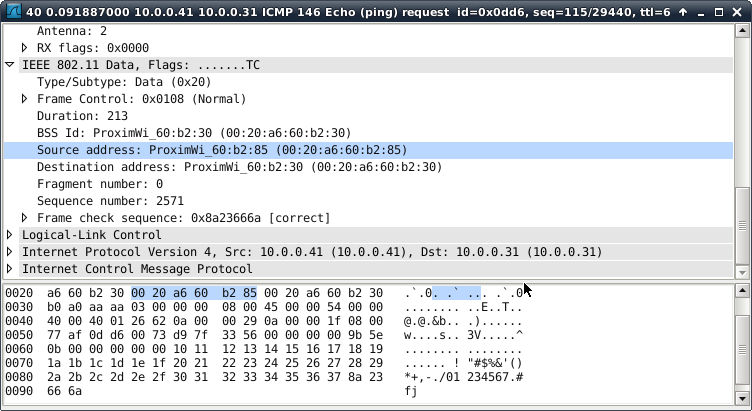
\includegraphics[width=\textwidth]{"images/other/im3.png}
		\caption{Finding the \emph{User's} \emph{MAC} address using \emph{Wireshark.}}
		\label{mac:wireshark}
	\end{figure}
	
	\begin{figure}
		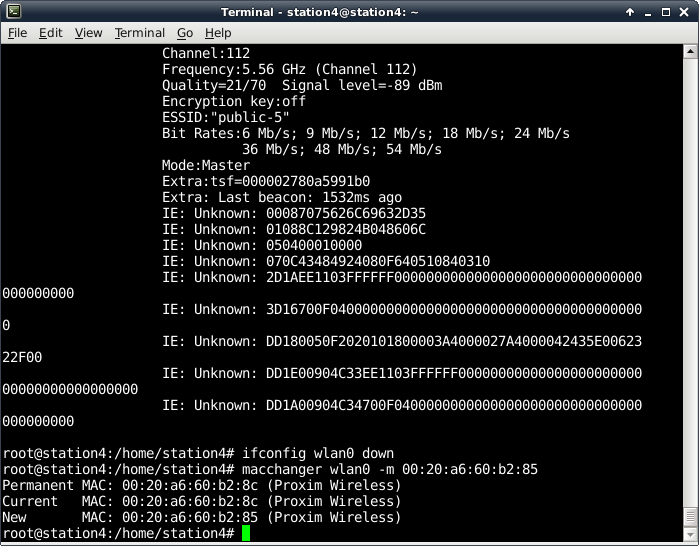
\includegraphics[width=\textwidth]{"images/other/im4.png}
		\caption{Changing the \emph{Attacker's} \emph{MAC} address using \emph{macchanger.}}
		\label{mac:changer}
	\end{figure}
	\subsubsection{Analysis}
		\emph{MAC} filtering can easily be bypassed with some limitations. The \emph{Attacker} does not get his own \emph{MAC} address, but share it with the \emph{User}, which leads to undesired side effects, such as both receiving the same packages. But it is very easily implemented and in wired networks it is harder for the \emph{Attacker} to sniff valid \emph{MAC} addresses.
	
  \subsection{Cracking WEP Encryption}
	\subsubsection{Running the Experiment}}


 \subsection{Breaking WPA2 Personal Passwords }
	\subsubsection{Running the Experiment}

\section{Analysis}
\bibliographystyle{plain}
\bibliography{bibliography}
\end{document}